\chapter{Experimentos}
\label{cap:capitulo6}

En este capítulo se recogen las distintos experimentos que se han llevado a cabo durante el desarrollo del proyecto. Estas pruebas han sido fundamentales para verificar el correcto funcionamiento del sistema de reconocimiento de maduración de frutos y su comunicación con el brazo robótico, permitiendo así alcanzar los objetivos definidos en fases anteriores del trabajo.

\section{Detección con YOLOv3 y PyTorch}
\label{exp_seleccion_algoritmo}

Dada la finalidad del proyecto, se requería que la detección de objetos se diera en tiempo real, por lo que se buscó información sobre YOLO, un sistema de código abierto que permitía esto a partir de una red neuronal convolucional para detectar objetos en imágenes y vídeo, y se iniciaron las pruebas pertinentes para la selección del algoritmo de detección y bibliotecas.\\

Después de realizar la lectura \textit{You Only Look Once: Unified, Real-Time Object Detection}\cite{Redmon16}, se replicó lo que se exponía en dicho artículo con la cámara integrada del ordenador portátil, mediante un programa en Python y usando la librería Open Source Computer Vision Library (OpenCV) mediante la biblioteca Pytorch. Este programa, partiendo del \textit{feed} de la propia webcam, descomponía el vídeo en imágenes o cuadros, alimentando a la red neuronal (en este caso YOLOv3), que recibía esta detección y se procesaba con OpenCV, dibujando los recuadros o \textit{bounding box} alrededor de los objetos que se detectaban en vivo.\\

Para ello, primero se realizó la instalación de Anaconda para poder crear un ambiente de trabajo independiente y así evitar problemas entre las versiones de los paquetes necesarios para la ejecución de estas pruebas, y posteriormente se instaló OpenCV. Se clonó el repositorio \textit{deteccion-objetos-video}\footnote{\url{https://github.com/puigalex/deteccion-objetos-video}} basado en el proyecto \textit{PyTorch-YOLOv3}\footnote{\url{https://github.com/eriklindernoren/PyTorch-YOLOv3}} para correr detección de objetos sobre video con el código y los actuales, mientras se siguieron los pasos detallados en el archivo README.
Una vez instalado todo, se probó a utilizar varios objetos y posteriormente varias frutas simultáneamente para verificar que el modelo las diferenciaba correctamente y las detectaba, tal y como se muestra en la Figura \ref{fig:Deteccion_Pytorch}.

  \begin{figure}[H]
    \begin{center}
      \subcapcentertrue
      \subfigure[Prueba deteccion de objetos con Pytorch]{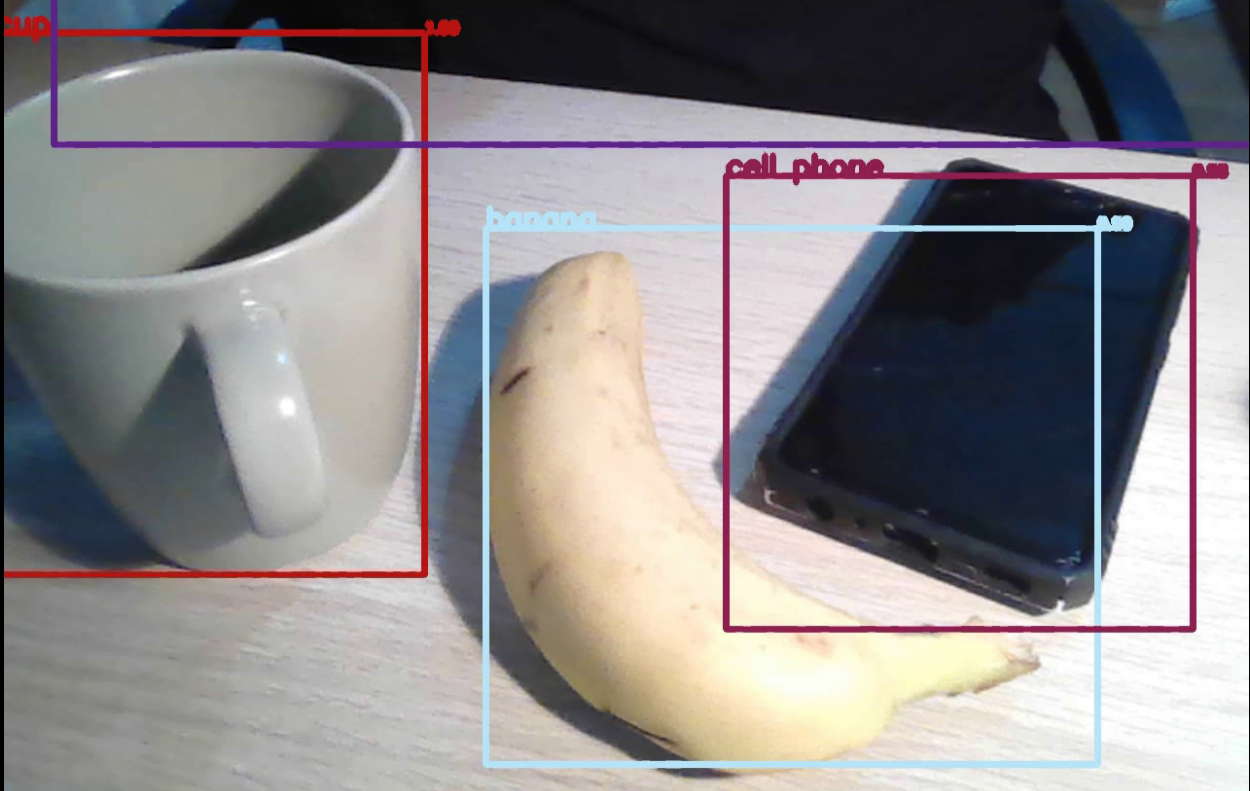
\includegraphics[width=73mm]{figs/Prueba deteccion de objetos con pytorch.png}}
      \hspace{2mm}
      \subfigure[Prueba deteccion de frutas con Pytorch]{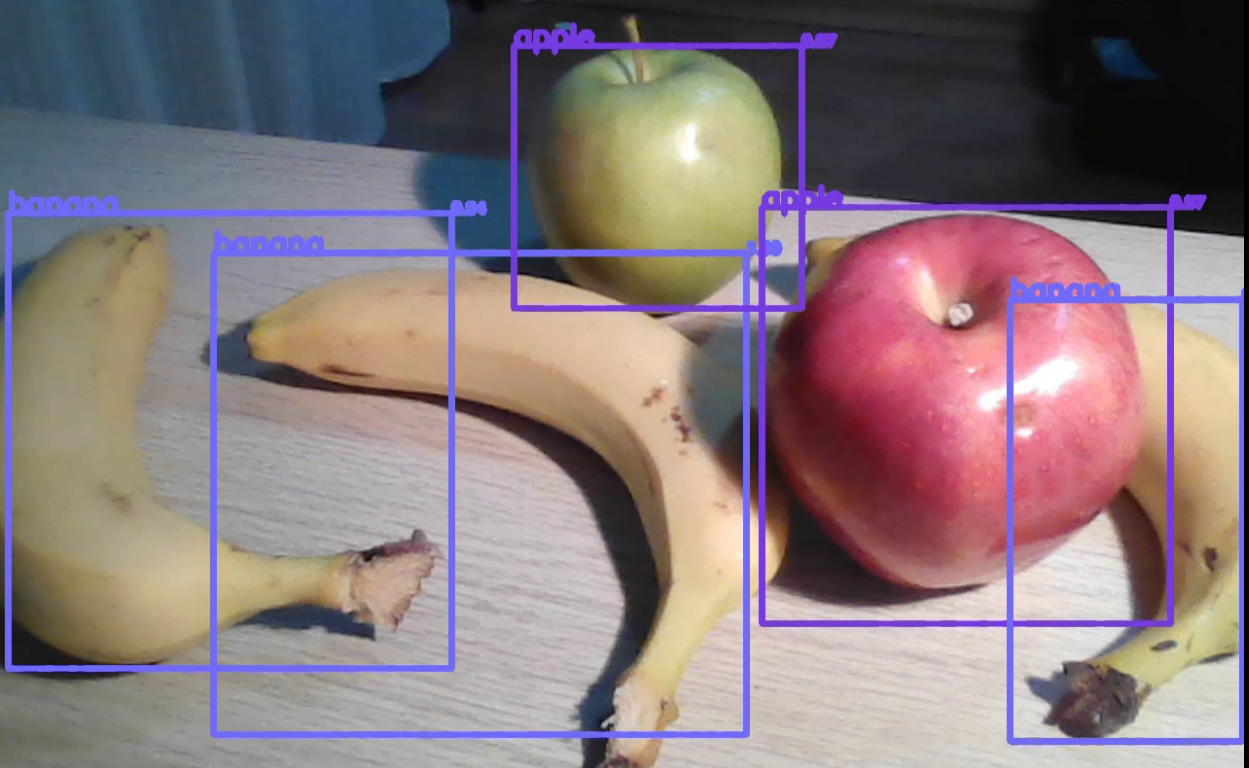
\includegraphics[width=75mm]{figs/Prueba derteccion de frutas con pytorch.png}}
    \end{center}
    \caption{Deteccion con Pytorch}
    \label{fig:Deteccion_Pytorch}
  \end{figure}

\section{Detección con YOLOv3 y TensorFlow}
\label{exp_seleccion_algoritmo}

Para poder comprobar las diferencias en un ejemplo práctico a la hora de detectar objetos entre PyTorch y TensorFlow, y de esta manera poder escoger una de las dos bibliotecas para el desarrollo del modelo de aprendizaje automático y aprendizaje profundo en este proyecto, se decidió crear de nuevo un entorno de Anaconda y probar a detectar objetos en imágenes utilizando Tensorflow.\\

Se utilizó el repositorio de \textit{deteccion\_objetos}\footnote{\url{https://github.com/puigalex/deteccion_objetos}} basados en la configuración \textit{faster rcnn resnet101 coco} de los modelos de detección de objetos de Tensorflow para poder llevar a cabo la comparación, y etiquetando imágenes, en este caso de tigres, mediante la herramienta labelImg\footnote{\url{https://github.com/HumanSignal/labelImg}}, se prepararon las carpetas y archivos de configuración correspondientes para poder llevar a cabo el entrenamiento del modelo siguiendo los pasos indicados en el repositorio utilizando una distribución de las imágenes utilizadas para el aprendizaje del modelo y su uso en la detecciónn aproximadamente del 70:30 (73\% datos de entrenamiento y 27\% datos de prueba)(Cuadro \ref{tab:Imagenes_Entrenamiento}) a partir de los cuales se entrenó ese 70\% con uno de los algoritmos y los respectivos parámetros escogidos y medimos su rendimiento usando el 30\% restante de los datos.

  \begin{table}[H]
  \centering
  \begin{tabularx}{\textwidth}{|X|X|X|}
    \hline
    \centering \textbf{Imágenes usadas en entrenamiento} & 
    \centering \textbf{Imágenes usadas en test} & 
    \centering \textbf{Número total de imágenes} \tabularnewline
    \hline
    \centering 594 & \centering 218 & \centering 812 \tabularnewline
    \hline
  \end{tabularx}
  \caption{Esta es una tabla de ejemplo con tabularx.}
  \label{tab:Imagenes_Entrenamiento}
  \end{table}

Se entrenó este modelo hasta que se observó que la pérdida estaba por debajo de 1, considerando que esta pérdida no era alta, y que no existían demasiadas fluctuaciones,  deteniendo este entrenamiento a los 1400 pasos, a pesar de que este entrenamiento estuviera programado para llegar hasta los 20000, ya que se trataba de una prueba simplemente, lo que supuso que se tuviera que utilizar el último checkpoint disponible, en este caso el del paso 1337 (Figura \ref{fig:Deteccion_Prueba_TF}), para convertirlo en un modelo final y de esta manera poder generar predicciones, utilizando imágenes de diferentes tamaños.

  \begin{figure}[H]
    \begin{center}
      \subcapcentertrue
      \subfigure[Pasos finales del entrenamiento con TensorFlow]{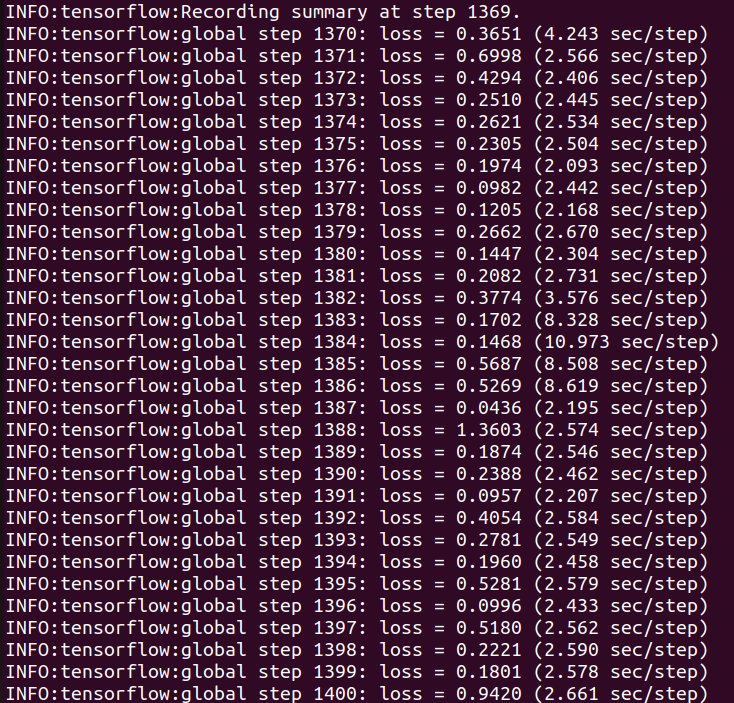
\includegraphics[height=50mm, width=70mm]{figs/Pasos finales del entrenamiento_TF.png}}
      \hspace{4mm}
      \subfigure[Checkpoints del entrenamiento con TensorFlow]{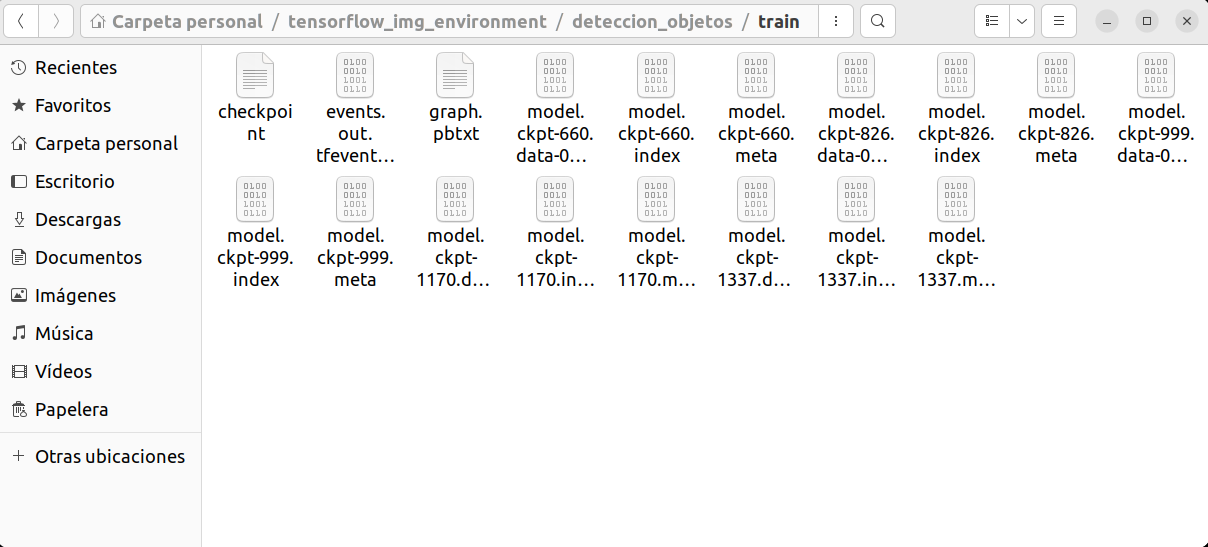
\includegraphics[height=50mm, width=70mm]{figs/checkpoints_TF.png}}
    \end{center}
    \caption{Entrenamiento del algoritmo con TensorFlow}
    \label{fig:Deteccion_Prueba_TF}
  \end{figure}
  
Una vez convertido el checkpoint en un modelo final, se procedió a realizar las primeras pruebas de detección en imágenes de este modelo, comprobando su capacidad para detectar correctamente los tigres para este caso, y evaluar visualmente los resultados obtenidos en algunos ejemplos mostrados en la Figura \ref{fig:deteccion_tensorflow_tigres}, de estas primeras detecciones realizadas tras el entrenamiento.

  \begin{figure}[H]
  \centering
  % Fila 1
  \begin{minipage}{0.46\textwidth}
    \centering
    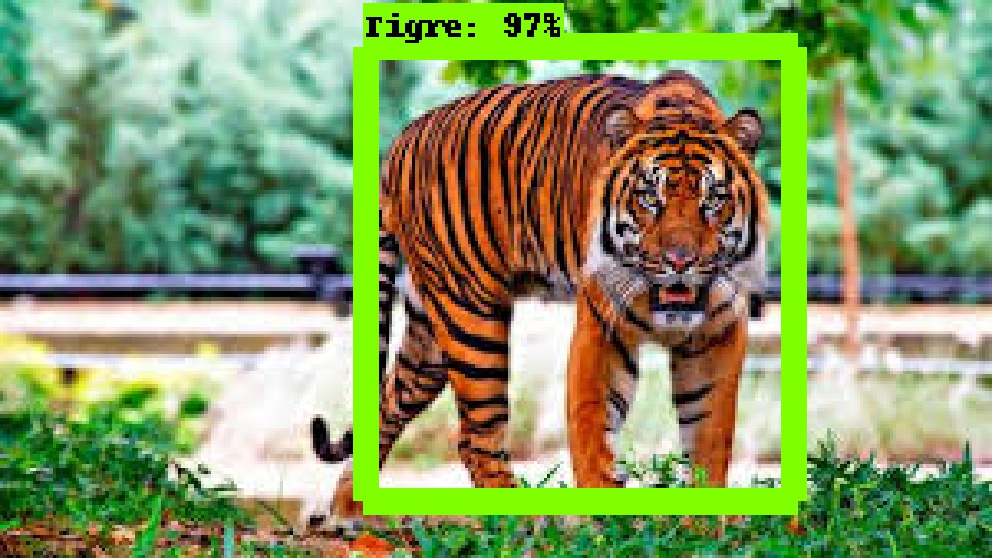
\includegraphics[width=\linewidth]{figs/tigre_1.jpeg}
  \end{minipage}
  \hspace{2mm}
  \begin{minipage}{0.46\textwidth}
    \centering
    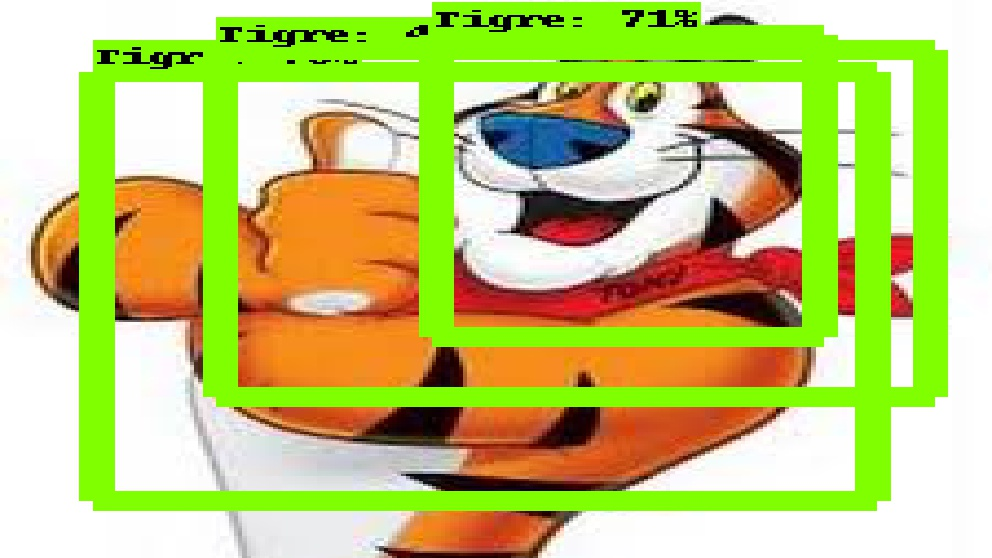
\includegraphics[width=\linewidth]{figs/tigre_2.jpeg}
  \end{minipage}
  \\[4mm] % Espacio vertical entre las dos filas
  % Fila 2
  \begin{minipage}{0.46\textwidth}
    \centering
    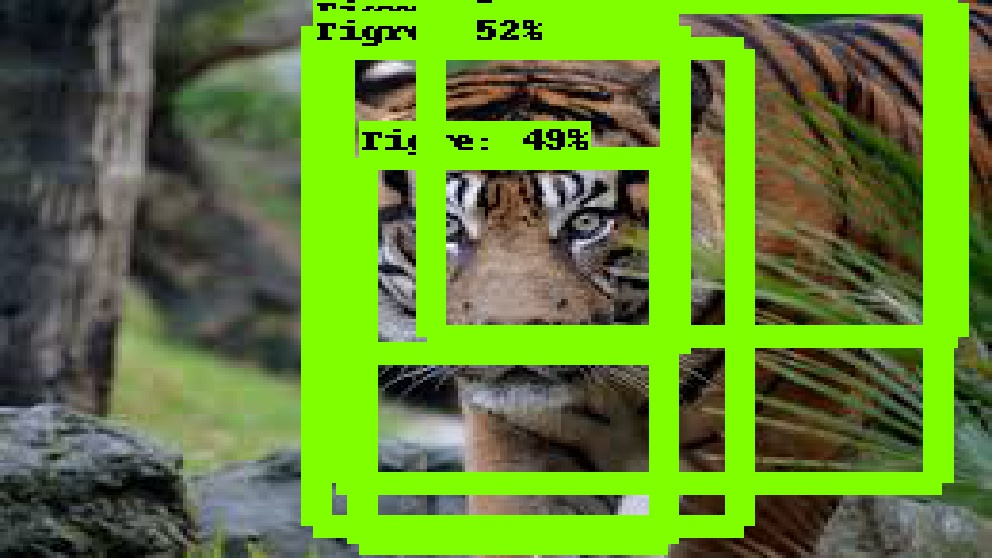
\includegraphics[width=\linewidth]{figs/tigre_4.jpeg}
  \end{minipage}
  \hspace{2mm}
  \begin{minipage}{0.46\textwidth}
    \centering
    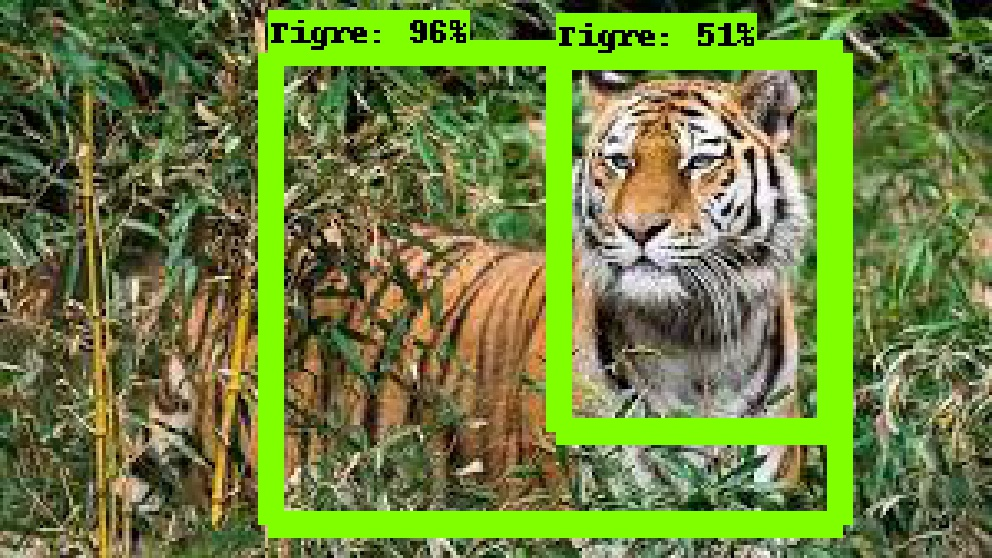
\includegraphics[width=\linewidth]{figs/tigre_5.jpeg}
  \end{minipage}
  \caption{Resultado de la detección en imágenes con TensorFlow}
  \label{fig:deteccion_tensorflow_tigres}
  \end{figure}
 
Dados los resultados obtenidos en las imágenes utilizadas para esta primera prueba, se decidió llevar a cabo un nuevo proceso de entrenamiento a partir del último checkpoint disponible con el objetivo principal de comprobar si, aumentando el número de pasos de entrenamiento, se lograba una mejora significativa tanto en la disminución del valor de pérdida como en el incremento del porcentaje de confianza en las detecciones realizadas. Así, se retomó el entrenamiento desde el checkpoint del paso 1337, extendiéndose en esta segunda ocasión hasta el paso 2945, momento en el cual se optó por detener manualmente el proceso al observarse una estabilización progresiva en los valores de pérdida, y siendo este último checkpoint generado fue el correspondiente al paso 2877, obteniéndose en este punto un valor de pérdida de tan solo 0.222, notablemente inferior al registrado en el primer intento. A continuación, se procedió a ejecutar nuevamente el programa sobre las mismas imágenes de prueba de tigres empleadas en la primera serie de tests, lo que permitió realizar una comparación directa entre ambos modelos, y observar que en esta segunda ejecución existía una clara mejora en la calidad de las detecciones, tanto en términos de mayor porcentaje de confianza como en la precisión de los cuadros delimitadores sobre los objetos detectados (ver Figura \ref{fig:deteccion_tensorflow_tigres_v2}).

  \begin{figure}[H]
  \centering
  % Fila 1
  \begin{minipage}{0.46\textwidth}
    \centering
    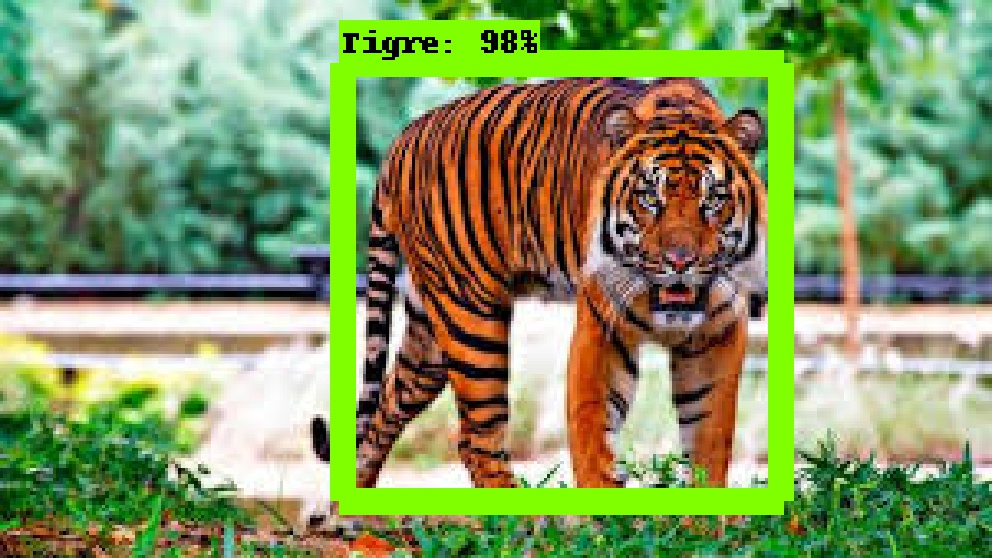
\includegraphics[width=\linewidth]{figs/tigre_1_v2.jpeg}
  \end{minipage}
  \hspace{2mm}
  \begin{minipage}{0.46\textwidth}
    \centering
    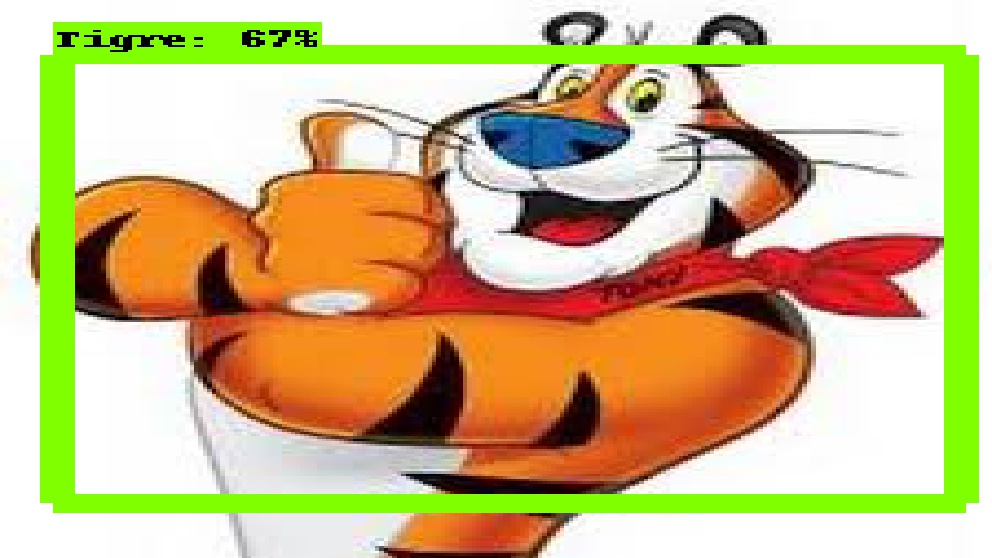
\includegraphics[width=\linewidth]{figs/tigre_2_v2.jpeg}
  \end{minipage}
  \\[4mm] % Espacio vertical entre las dos filas
  % Fila 2
  \begin{minipage}{0.46\textwidth}
    \centering
    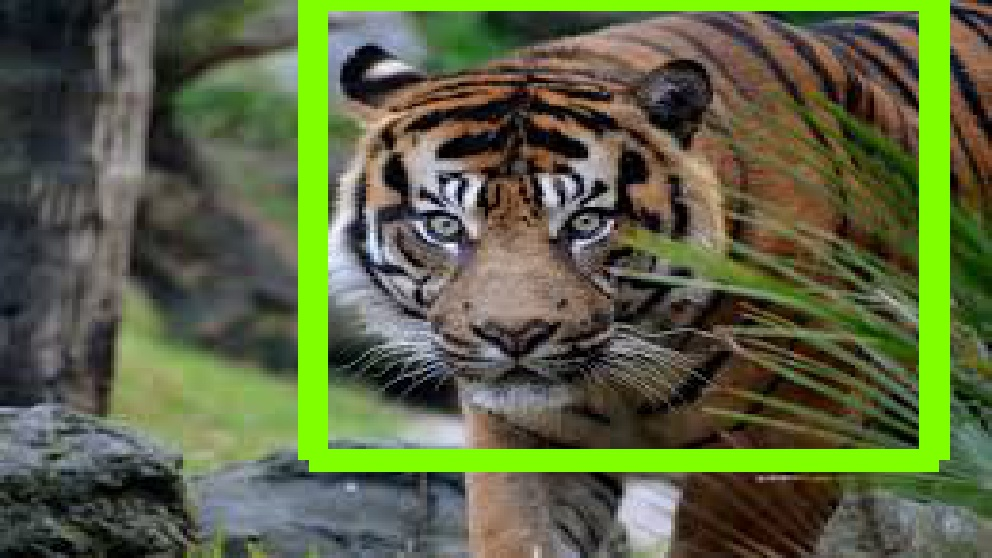
\includegraphics[width=\linewidth]{figs/tigre_4_v2.jpeg}
  \end{minipage}
  \hspace{2mm}
  \begin{minipage}{0.46\textwidth}
    \centering
    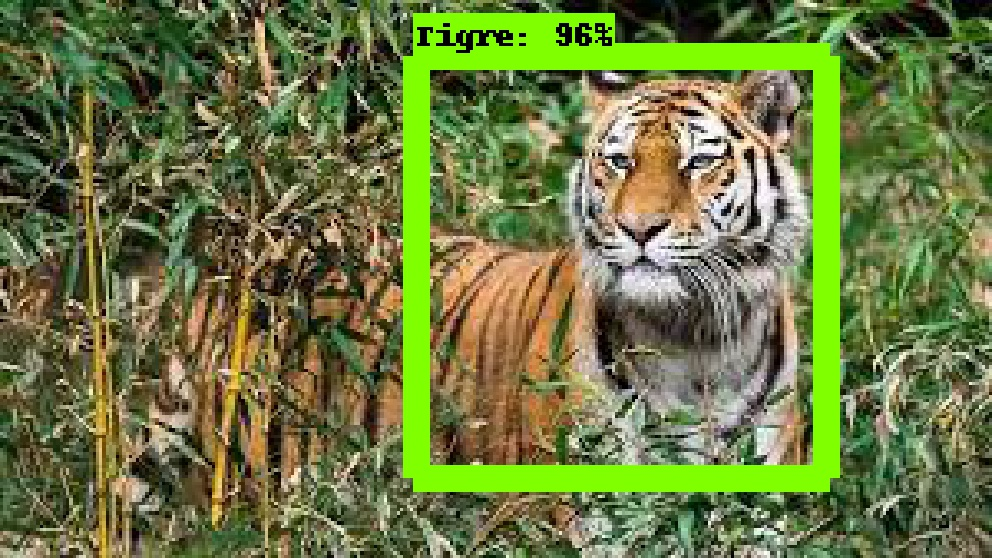
\includegraphics[width=\linewidth]{figs/tigre_5_v2.jpeg}
  \end{minipage}
  \caption{Resultado del reentrenamiento de la detección en imágenes con TensorFlow}
  \label{fig:deteccion_tensorflow_tigres_v2}
  \end{figure}


Después de llevar a cabo estas poruebas con el ejemplo de los tigres, se comprobó si el modelo funcionaría también con el objeto final, en este caso, con fresas, por lo que, a través de la página Kaggle, se obtuvo un dataset de 262 frutas\footnote{\url{https://www.kaggle.com/datasets/aelchimminut/fruits262}} de las cuales únicamente se utilizó el archivo de las fresas, que contenía 1002 imágenes para llevar a cabo estas pruebas.\\

Una vez descargado el archivo, se comenzó a etiquetar una a una las imágenes mediante la herramienta labelImg para obtener los archivos xml, tal y como se había hecho con el ejemplo anterior de los tigres, y antes de terminar de etiquetar el dataset entero, se probó este modelo utlizando las primeras 405 imágenes etiquetadas siguiendo una distribución de estas del 80:20 para su entrenamiento y usando el checkpoint guardado en el paso 3490 para congelar el modelo, y así poder utilizar varias imágenes aún por etiquetar para probarlo, obteniendo un resultado satisfactorio en cuanto a la detección y su confianza, tal y como se puede observar en la Figura \ref{fig:Deteccion_Fresas_Imagenes_TF}.

  \begin{figure}[H]
  \centering
  % Fila 1
  \begin{minipage}{0.45\textwidth}
    \centering
    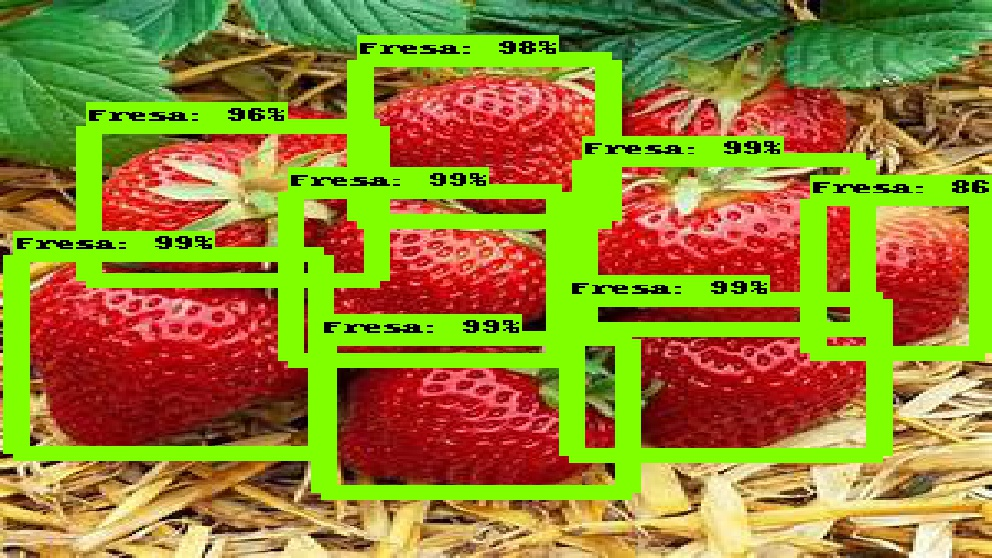
\includegraphics[width=\linewidth]{figs/999.jpeg}
  \end{minipage}
  \hspace{2mm}
  \begin{minipage}{0.45\textwidth}
    \centering
    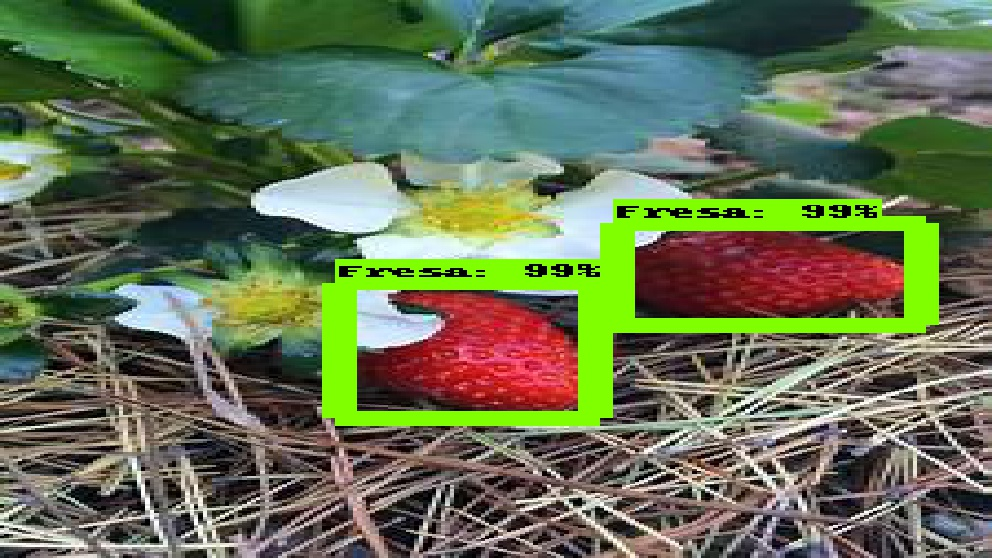
\includegraphics[width=\linewidth]{figs/947.jpeg}
  \end{minipage}
  \\[4mm] % Espacio vertical entre las dos filas
  % Fila 2
  \begin{minipage}{0.45\textwidth}
    \centering
    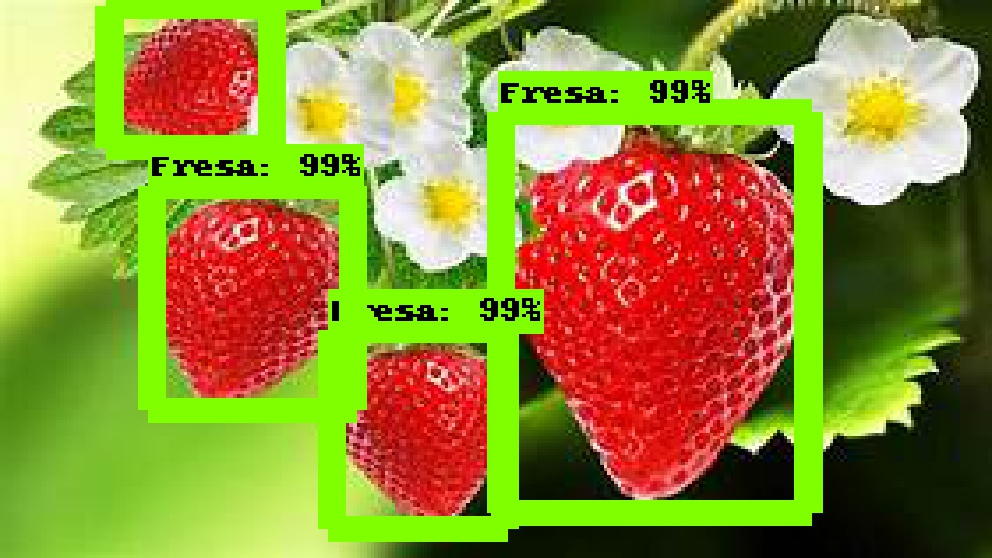
\includegraphics[width=\linewidth]{figs/868.jpeg}
  \end{minipage}
  \hspace{2mm}
  \begin{minipage}{0.45\textwidth}
    \centering
    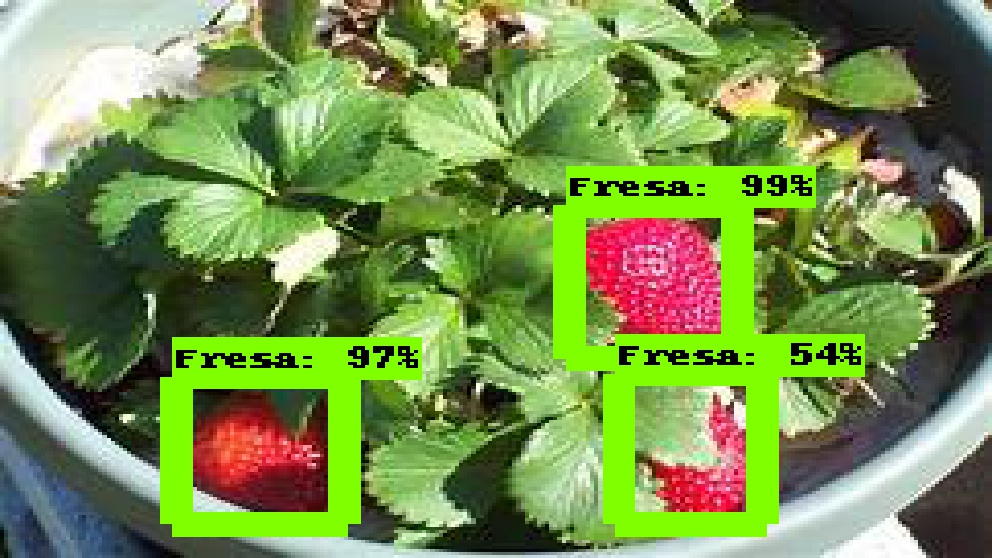
\includegraphics[width=\linewidth]{figs/1000.jpeg}
  \end{minipage}
  \caption{Pruebas de deteccion de fresas en imágenes con TensorFlow}
  \label{fig:Deteccion_Fresas_Imagenes_TF}
  \end{figure}

Tras haber conseguido la detección de fresas en imágenes estáticas utilizando TensorFlow, el siguiente paso dentro del desarrollo del sistema consistió en extender las pruebas a la detección en vídeo en tiempo real, por lo que, de forma análoga a como se había realizado previamente con la librería PyTorch, se procedió a evaluar distintos modelos de detección de objetos pertenecientes al zoo de TensorFlow (TensorFlow 2 Detection Model Zoo), los cuales, al estar ya preentrenados sobre conjuntos de datos de referencia, permitieron llevar a cabo una comparación de estos diferentes modelos o sistemas bajo las mismas condiciones iniciales sin necesidad de realizar un nuevo entrenamiento desde cero. Para la realización de estas pruebas, se utilizó tanto la cámara web integrada del ordenador portátil como una imagen previamente seleccionada, para que, de esta manera pudieran observarse las diferencias entre los modelos tanto en la detección en vídeo como en la detección en imágenes, y poder valorar qué modelo de los tres distintos probados ofrecería mejores prestaciones en términos de precisión, velocidad de procesamiento y robustez frente a las condiciones reales de trabajo (ver Figuras  \ref{fig:modelo_ssd_mobilenet}, \ref{fig:modelo_efficientdet_d4} y \ref{fig:modelo_faster_rcnn_resnet50}). 

	\begin{figure}[H]
    		\begin{center}
      		\subcapcentertrue
      		\subfigure[Resultado del modelo en imagen]{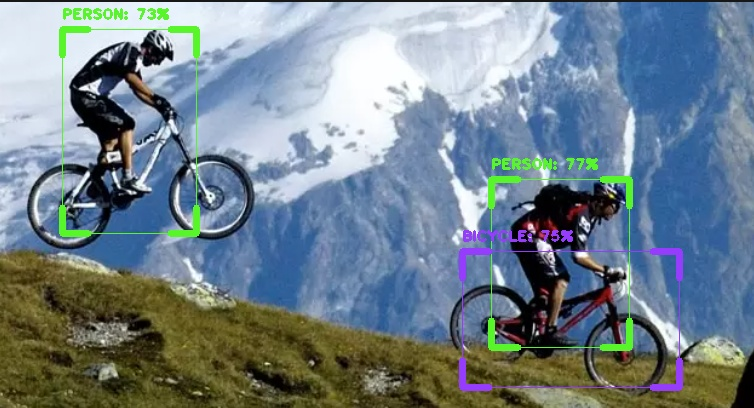
\includegraphics[height=50mm, width=70mm]{figs/ssd_mobilenet_v2_320x320_coco17_tpu-8.jpeg}}
      		\hspace{2mm}
      		\subfigure[Resultado del modelo en vídeo]{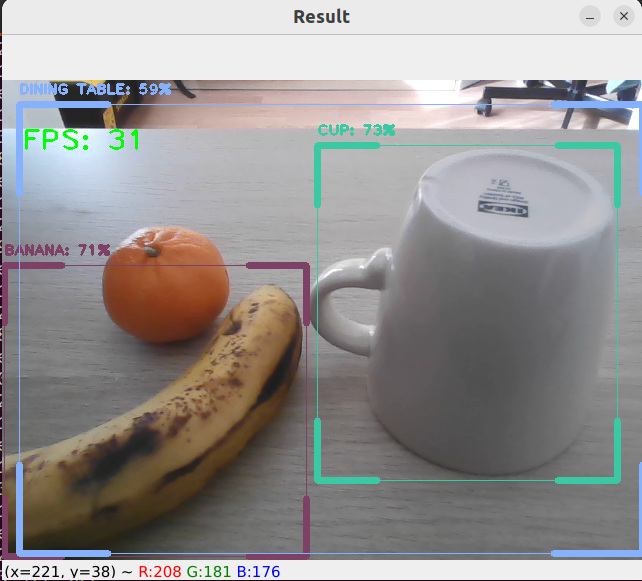
\includegraphics[height=50mm, width=70mm]{figs/webcam ssd_mobilenet_v2_320x320_coco17_tpu-8.png}}
    	\end{center}
    	\caption{Modelo ssd\_mobilenet\_v2\_320x320\_coco17\_tpu-8}
    	\label{fig:modelo_ssd_mobilenet}
  	\end{figure}
  	

  	\begin{figure}[H]
    		\begin{center}
      		\subcapcentertrue
      		\subfigure[Resultado del modelo en imagen]{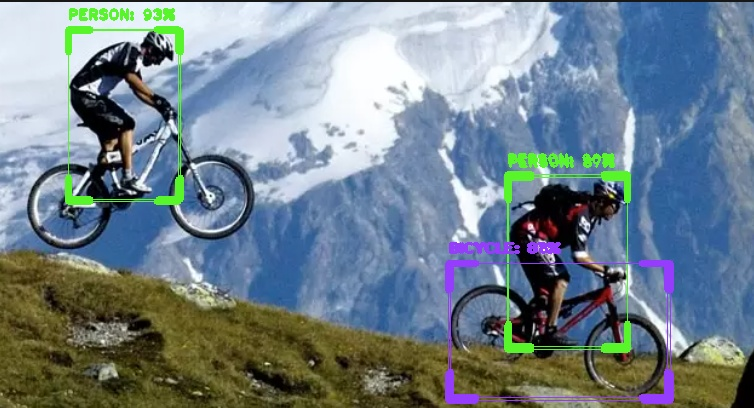
\includegraphics[height=50mm, width=70mm]{figs/efficientdet_d4_coco17_tpu-32.jpeg}}
      		\hspace{2mm}
      		\subfigure[Resultado del modelo en vídeo]{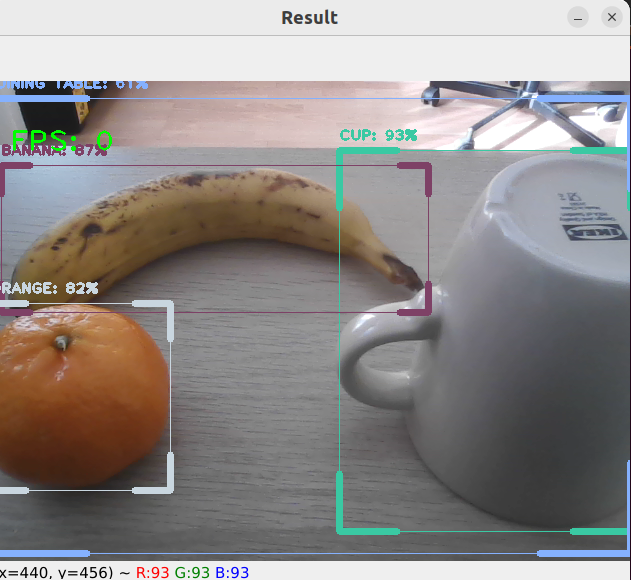
\includegraphics[height=50mm, width=70mm]{figs/webcam efficientdet_d4_coco17_tpu-32.png}}
    	\end{center}
    	\caption{Modelo efficientdet\_d4\_coco17\_tpu-32}
    	\label{fig:modelo_efficientdet_d4}
  	\end{figure}

  	\begin{figure}[H]
    		\begin{center}
      		\subcapcentertrue
      		\subfigure[Resultado del modelo en imagen]{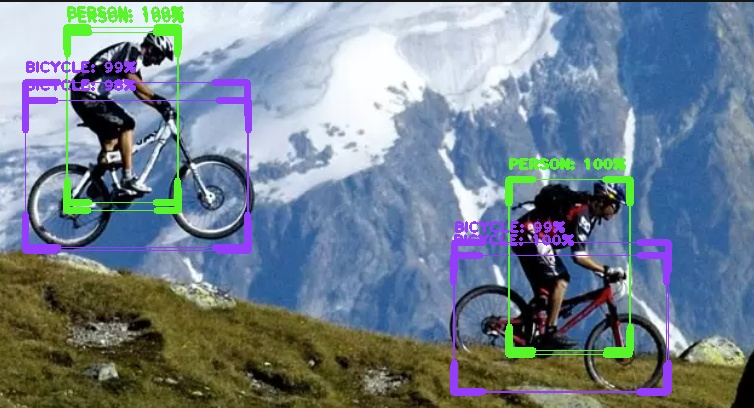
\includegraphics[height=50mm, width=70mm]{figs/faster_rcnn_resnet50_v1_640x640_coco17_tpu-8.jpeg}}
      		\hspace{2mm}
      		\subfigure[Resultado del modelo en vídeo]{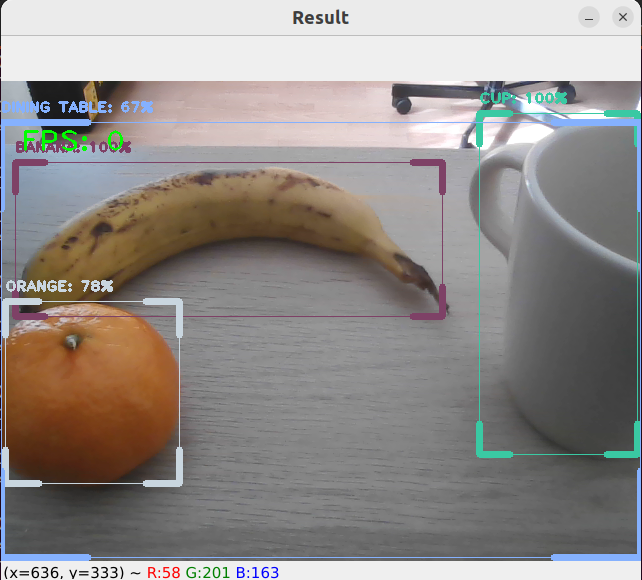
\includegraphics[height=50mm, width=70mm]{figs/webcam faster_rcnn_resnet50_v1_640x640_coco17_tpu-8.png}}
    	\end{center}
    	\caption{Modelo faster\_rcnn\_resnet50\_v1\_640x640\_coco17\_tpu-8 }
    	\label{fig:modelo_faster_rcnn_resnet50}
  	\end{figure}	
  	
\pagebreak
Después de haber llevado a cabo estas pruebas con los modelos de detección de objetos ssd\_mobilenet\_v2\_320x320\_coco17\_tpu-8, efficientdet\_d4\_coco17\_tpu-32 y faster\_rcnn\_resnet50\_v1\_640x640\_coco17\_tpu-8, y tras valorar que, el principal uso del modelo en la aplicación final sería la de llevar a cabo detecciones a tiempo real con una cámara, se escogió el modelo ssd\_mobilenet\_v2 para proseguir con los experimentos, incluso por delante de cualquiera de los otros dos modelos, incluso teniendo menor precisión y calidad de detección, ya que destacaba principalmente por su elevada velocidad de procesamiento y su bajo consumo de recursos, gracias a su arquitectura ligera basada en MobileNetV2 y su tamaño de entrada reducido, haciéndolo especialmente adecuado para aplicaciones en tiempo real sobre hardware con capacidades limitadas, como puede ser un sistema de visión embarcado en un brazo robótico.\\

Para ello, y dado que para poder llevar a cabo la detección de fresas era necesario utilizar un modelo entrenado desde cero, tal y como muestra la Figura \ref{fig:entrenamiento_ssdmobilenet}, se utilizó de guía el repositorio \textit{real\_time\_object\_detection\_cpu}\footnote{\url{https://github.com/haroonshakeel/real_time_object_detection_cpu/blob/main/README.md}}, creando y activando un nuevo entorno de Anaconda, donde se instalaron los paquetes y librerías necesarios para ello junto al Object Detection API de TensorFlow junto con Jupyter Notebook\footnote{\url{https://jupyter.org}}, un entorno computacional interactivo basado en web para crear cuadernos que contienen código en vivo, ecuaciones, visualizaciones y texto narrativo. 

 \begin{figure} [H]
  \begin{center}
    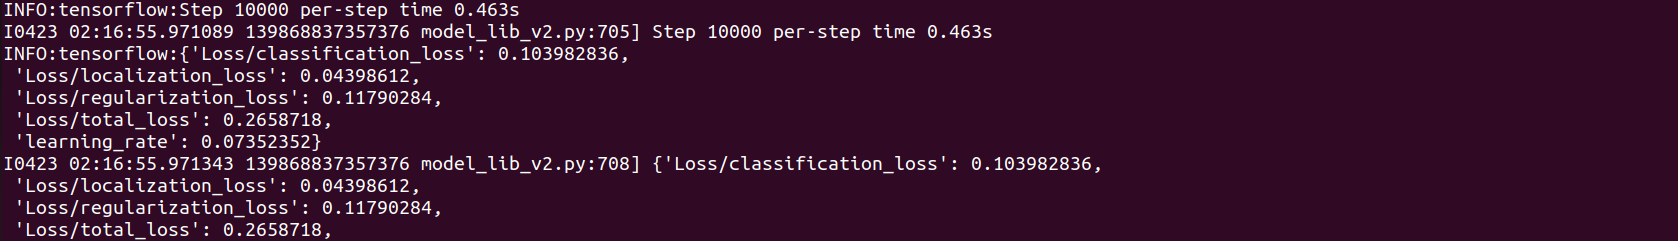
\includegraphics[width=150mm]{figs/tensorflow step 10000.png}
  \end{center}
  \caption{Entrenamiento del modelo ssd\_mobilenet\_v2 para detectar fresas}
  \label{fig:entrenamiento_ssdmobilenet}
 \end{figure}

Completada la configuración del entorno, la instalación de todos los componentes, y el entrenamiento del modelo, se realizó una primera prueba de detección utilizando el modelo entrenado para comprobar si funcionaba, obteniendo las primeras predicciones en tiempo real sobre vídeo con fresas reales, y de este modo, poder llevar a cabo la batería de pruebas en las cuales se variaba tanto el número de fresas como las condiciones de luz, siendo los resultados de estos escenarios los que se muestran a continuación:
\pagebreak

\begin{figure}[H]
  \centering

  % Fila 1
  \subfigure[Detección de una única fresa con luz natural de día]{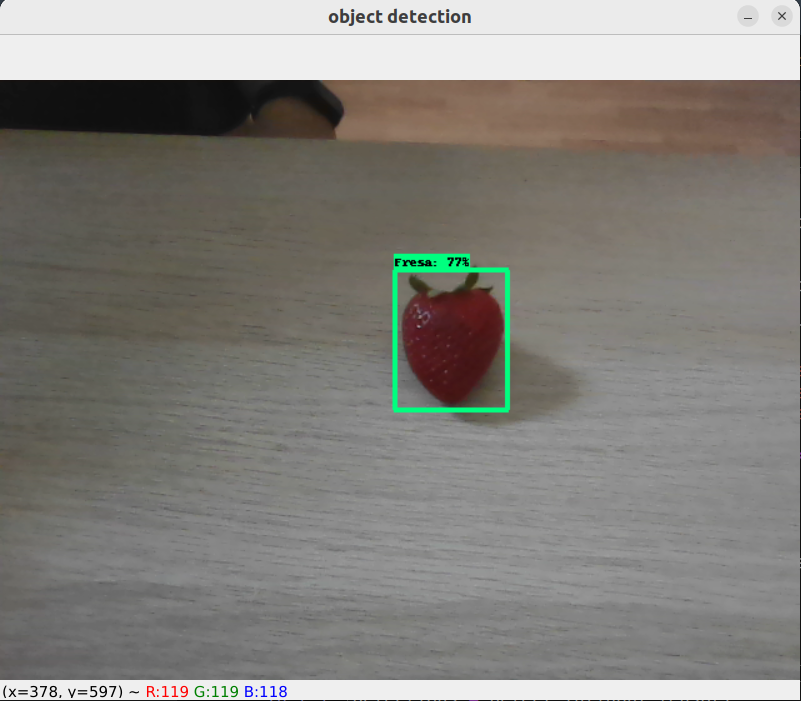
\includegraphics[width=0.30\textwidth]{figs/Deteccion una fresa luz natural dia JN.png}}
  \hspace{5mm}
  \subfigure[Segunda imagen]{\includegraphics[width=0.30\textwidth]{ruta/imagen2.jpg}}
  \hspace{5mm}
  \subfigure[Tercera imagen]{\includegraphics[width=0.30\textwidth]{ruta/imagen3.jpg}}

  \\[5mm] % Espacio vertical entre filas  

  % Fila 2
  \subfigure[Cuarta imagen]{\includegraphics[width=0.30\textwidth]{ruta/imagen4.jpg}}
  \hspace{5mm}
  \subfigure[Quinta imagen]{\includegraphics[width=0.30\textwidth]{ruta/imagen5.jpg}}
  \hspace{5mm}
  \subfigure[Sexta imagen]{\includegraphics[width=0.30\textwidth]{ruta/imagen6.jpg}}
  \caption{Collage de 6 imágenes en dos filas}
  \label{fig:collage_6}
\end{figure}







\begin{itemize}
	\item{Detección de una única fresa con luz natural de día:} 
	\item{Detección de varias fresas con luz natural de día:}
	\item{Detección de una única fresa con luz artifical de día:} 
	\item{Detección de varias fresas con luz artifical de día:} 
	\item{Detección de una única fresa con luz artifical de noche:}
	\item{Detección de varias fresas con luz artifical de noche:} 

\end{itemize}








